\documentclass[1p]{elsarticle_modified}
%\bibliographystyle{elsarticle-num}

%\usepackage[colorlinks]{hyperref}
%\usepackage{abbrmath_seonhwa} %\Abb, \Ascr, \Acal ,\Abf, \Afrak
\usepackage{amsfonts}
\usepackage{amssymb}
\usepackage{amsmath}
\usepackage{amsthm}
\usepackage{scalefnt}
\usepackage{amsbsy}
\usepackage{kotex}
\usepackage{caption}
\usepackage{subfig}
\usepackage{color}
\usepackage{graphicx}
\usepackage{xcolor} %% white, black, red, green, blue, cyan, magenta, yellow
\usepackage{float}
\usepackage{setspace}
\usepackage{hyperref}

\usepackage{tikz}
\usetikzlibrary{arrows}

\usepackage{multirow}
\usepackage{array} % fixed length table
\usepackage{hhline}

%%%%%%%%%%%%%%%%%%%%%
\makeatletter
\renewcommand*\env@matrix[1][\arraystretch]{%
	\edef\arraystretch{#1}%
	\hskip -\arraycolsep
	\let\@ifnextchar\new@ifnextchar
	\array{*\c@MaxMatrixCols c}}
\makeatother %https://tex.stackexchange.com/questions/14071/how-can-i-increase-the-line-spacing-in-a-matrix
%%%%%%%%%%%%%%%

\usepackage[normalem]{ulem}

\newcommand{\msout}[1]{\ifmmode\text{\sout{\ensuremath{#1}}}\else\sout{#1}\fi}
%SOURCE: \msout is \stkout macro in https://tex.stackexchange.com/questions/20609/strikeout-in-math-mode

\newcommand{\cancel}[1]{
	\ifmmode
	{\color{red}\msout{#1}}
	\else
	{\color{red}\sout{#1}}
	\fi
}

\newcommand{\add}[1]{
	{\color{blue}\uwave{#1}}
}

\newcommand{\replace}[2]{
	\ifmmode
	{\color{red}\msout{#1}}{\color{blue}\uwave{#2}}
	\else
	{\color{red}\sout{#1}}{\color{blue}\uwave{#2}}
	\fi
}

\newcommand{\Sol}{\mathcal{S}} %segment
\newcommand{\D}{D} %diagram
\newcommand{\A}{\mathcal{A}} %arc


%%%%%%%%%%%%%%%%%%%%%%%%%%%%%5 test

\def\sl{\operatorname{\textup{SL}}(2,\Cbb)}
\def\psl{\operatorname{\textup{PSL}}(2,\Cbb)}
\def\quan{\mkern 1mu \triangleright \mkern 1mu}

\theoremstyle{definition}
\newtheorem{thm}{Theorem}[section]
\newtheorem{prop}[thm]{Proposition}
\newtheorem{lem}[thm]{Lemma}
\newtheorem{ques}[thm]{Question}
\newtheorem{cor}[thm]{Corollary}
\newtheorem{defn}[thm]{Definition}
\newtheorem{exam}[thm]{Example}
\newtheorem{rmk}[thm]{Remark}
\newtheorem{alg}[thm]{Algorithm}

\newcommand{\I}{\sqrt{-1}}
\begin{document}

%\begin{frontmatter}
%
%\title{Boundary parabolic representations of knots up to 8 crossings}
%
%%% Group authors per affiliation:
%\author{Yunhi Cho} 
%\address{Department of Mathematics, University of Seoul, Seoul, Korea}
%\ead{yhcho@uos.ac.kr}
%
%
%\author{Seonhwa Kim} %\fnref{s_kim}}
%\address{Center for Geometry and Physics, Institute for Basic Science, Pohang, 37673, Korea}
%\ead{ryeona17@ibs.re.kr}
%
%\author{Hyuk Kim}
%\address{Department of Mathematical Sciences, Seoul National University, Seoul 08826, Korea}
%\ead{hyukkim@snu.ac.kr}
%
%\author{Seokbeom Yoon}
%\address{Department of Mathematical Sciences, Seoul National University, Seoul, 08826,  Korea}
%\ead{sbyoon15@snu.ac.kr}
%
%\begin{abstract}
%We find all boundary parabolic representation of knots up to 8 crossings.
%
%\end{abstract}
%\begin{keyword}
%    \MSC[2010] 57M25 
%\end{keyword}
%
%\end{frontmatter}

%\linenumbers
%\tableofcontents
%
\newcommand\colored[1]{\textcolor{white}{\rule[-0.35ex]{0.8em}{1.4ex}}\kern-0.8em\color{red} #1}%
%\newcommand\colored[1]{\textcolor{white}{ #1}\kern-2.17ex	\textcolor{white}{ #1}\kern-1.81ex	\textcolor{white}{ #1}\kern-2.15ex\color{red}#1	}

{\Large $\underline{12n_{0357}~(K12n_{0357})}$}

\setlength{\tabcolsep}{10pt}
\renewcommand{\arraystretch}{1.6}
\vspace{1cm}\begin{tabular}{m{100pt}>{\centering\arraybackslash}m{274pt}}
\multirow{5}{120pt}{
	\centering
	\includegraphics[width=112pt]{../../../GIT/diagram.site/Diagrams/png/2446_12n_0357.png}\\
\ \ \ A knot diagram\footnotemark}&
\allowdisplaybreaks
\textbf{Linearized knot diagam} \\
\cline{2-2}
 &
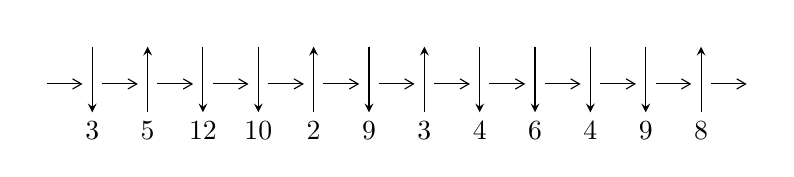
\begin{tikzpicture}[x=20pt, y=17pt]
	% nodes
	\node (C0) at (0, 0) {};
	\node (C1) at (1, 0) {};
	\node (C1U) at (1, +1) {};
	\node (C1D) at (1, -1) {3};

	\node (C2) at (2, 0) {};
	\node (C2U) at (2, +1) {};
	\node (C2D) at (2, -1) {5};

	\node (C3) at (3, 0) {};
	\node (C3U) at (3, +1) {};
	\node (C3D) at (3, -1) {12};

	\node (C4) at (4, 0) {};
	\node (C4U) at (4, +1) {};
	\node (C4D) at (4, -1) {10};

	\node (C5) at (5, 0) {};
	\node (C5U) at (5, +1) {};
	\node (C5D) at (5, -1) {2};

	\node (C6) at (6, 0) {};
	\node (C6U) at (6, +1) {};
	\node (C6D) at (6, -1) {9};

	\node (C7) at (7, 0) {};
	\node (C7U) at (7, +1) {};
	\node (C7D) at (7, -1) {3};

	\node (C8) at (8, 0) {};
	\node (C8U) at (8, +1) {};
	\node (C8D) at (8, -1) {4};

	\node (C9) at (9, 0) {};
	\node (C9U) at (9, +1) {};
	\node (C9D) at (9, -1) {6};

	\node (C10) at (10, 0) {};
	\node (C10U) at (10, +1) {};
	\node (C10D) at (10, -1) {4};

	\node (C11) at (11, 0) {};
	\node (C11U) at (11, +1) {};
	\node (C11D) at (11, -1) {9};

	\node (C12) at (12, 0) {};
	\node (C12U) at (12, +1) {};
	\node (C12D) at (12, -1) {8};
	\node (C13) at (13, 0) {};

	% arrows
	\draw[->,>={angle 60}]
	(C0) edge (C1) (C1) edge (C2) (C2) edge (C3) (C3) edge (C4) (C4) edge (C5) (C5) edge (C6) (C6) edge (C7) (C7) edge (C8) (C8) edge (C9) (C9) edge (C10) (C10) edge (C11) (C11) edge (C12) (C12) edge (C13) ;	\draw[->,>=stealth]
	(C1U) edge (C1D) (C2D) edge (C2U) (C3U) edge (C3D) (C4U) edge (C4D) (C5D) edge (C5U) (C6U) edge (C6D) (C7D) edge (C7U) (C8U) edge (C8D) (C9U) edge (C9D) (C10U) edge (C10D) (C11U) edge (C11D) (C12D) edge (C12U) ;
	\end{tikzpicture} \\
\hhline{~~} \\& 
\textbf{Solving Sequence} \\ \cline{2-2} 
 &
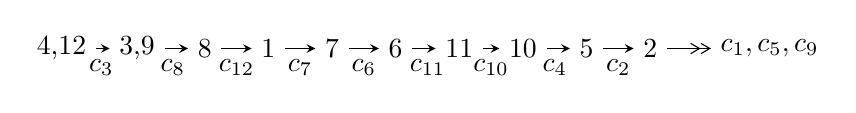
\begin{tikzpicture}[x=23pt, y=7pt]
	% node
	\node (A0) at (-1/8, 0) {4,12};
	\node (A1) at (17/16, 0) {3,9};
	\node (A2) at (17/8, 0) {8};
	\node (A3) at (25/8, 0) {1};
	\node (A4) at (33/8, 0) {7};
	\node (A5) at (41/8, 0) {6};
	\node (A6) at (49/8, 0) {11};
	\node (A7) at (57/8, 0) {10};
	\node (A8) at (65/8, 0) {5};
	\node (A9) at (73/8, 0) {2};
	\node (C1) at (1/2, -1) {$c_{3}$};
	\node (C2) at (13/8, -1) {$c_{8}$};
	\node (C3) at (21/8, -1) {$c_{12}$};
	\node (C4) at (29/8, -1) {$c_{7}$};
	\node (C5) at (37/8, -1) {$c_{6}$};
	\node (C6) at (45/8, -1) {$c_{11}$};
	\node (C7) at (53/8, -1) {$c_{10}$};
	\node (C8) at (61/8, -1) {$c_{4}$};
	\node (C9) at (69/8, -1) {$c_{2}$};
	\node (A10) at (11, 0) {$c_{1},c_{5},c_{9}$};

	% edge
	\draw[->,>=stealth]	
	(A0) edge (A1) (A1) edge (A2) (A2) edge (A3) (A3) edge (A4) (A4) edge (A5) (A5) edge (A6) (A6) edge (A7) (A7) edge (A8) (A8) edge (A9) ;
	\draw[->>,>={angle 60}]	
	(A9) edge (A10);
\end{tikzpicture} \\ 

\end{tabular} \\

\footnotetext{
The image of knot diagram is generated by the software ``\textbf{Draw programme}" developed by Andrew Bartholomew(\url{http://www.layer8.co.uk/maths/draw/index.htm\#Running-draw}), where we modified some parts for our purpose(\url{https://github.com/CATsTAILs/LinksPainter}).
}\phantom \\ \newline 
\centering \textbf{Ideals for irreducible components\footnotemark of $X_{\text{par}}$} 
 
\begin{align*}
I^u_{1}&=\langle 
1.81165\times10^{192} u^{72}-4.45965\times10^{192} u^{71}+\cdots+9.74080\times10^{191} b+1.06210\times10^{193},\\
\phantom{I^u_{1}}&\phantom{= \langle  }-9.93968\times10^{192} u^{72}+2.39622\times10^{193} u^{71}+\cdots+2.92224\times10^{192} a-7.03543\times10^{193},\;u^{73}-3 u^{72}+\cdots+u-3\rangle \\
I^u_{2}&=\langle 
377188189 u^{23}+1378863855 u^{22}+\cdots+61167471 b+138784360,\\
\phantom{I^u_{2}}&\phantom{= \langle  }-64492387 u^{23}-295831704 u^{22}+\cdots+61167471 a-153446503,\;u^{24}+4 u^{23}+\cdots- u^3+1\rangle \\
\\
\end{align*}
\raggedright * 2 irreducible components of $\dim_{\mathbb{C}}=0$, with total 97 representations.\\
\footnotetext{All coefficients of polynomials are rational numbers. But the coefficients are sometimes approximated in decimal forms when there is not enough margin.}
\newpage
\renewcommand{\arraystretch}{1}
\centering \section*{I. $I^u_{1}= \langle 1.81\times10^{192} u^{72}-4.46\times10^{192} u^{71}+\cdots+9.74\times10^{191} b+1.06\times10^{193},\;-9.94\times10^{192} u^{72}+2.40\times10^{193} u^{71}+\cdots+2.92\times10^{192} a-7.04\times10^{193},\;u^{73}-3 u^{72}+\cdots+u-3 \rangle$}
\flushleft \textbf{(i) Arc colorings}\\
\begin{tabular}{m{7pt} m{180pt} m{7pt} m{180pt} }
\flushright $a_{4}=$&$\begin{pmatrix}1\\0\end{pmatrix}$ \\
\flushright $a_{12}=$&$\begin{pmatrix}0\\u\end{pmatrix}$ \\
\flushright $a_{3}=$&$\begin{pmatrix}1\\- u^2\end{pmatrix}$ \\
\flushright $a_{9}=$&$\begin{pmatrix}3.40139 u^{72}-8.19995 u^{71}+\cdots+26.4023 u+24.0755\\-1.85986 u^{72}+4.57832 u^{71}+\cdots-12.4794 u-10.9036\end{pmatrix}$ \\
\flushright $a_{8}=$&$\begin{pmatrix}1.54153 u^{72}-3.62163 u^{71}+\cdots+13.9229 u+13.1719\\-1.85986 u^{72}+4.57832 u^{71}+\cdots-12.4794 u-10.9036\end{pmatrix}$ \\
\flushright $a_{1}=$&$\begin{pmatrix}0.412176 u^{72}-0.538736 u^{71}+\cdots-4.02065 u+8.34606\\-0.637800 u^{72}+1.60567 u^{71}+\cdots-1.74620 u-1.17888\end{pmatrix}$ \\
\flushright $a_{7}=$&$\begin{pmatrix}3.10355 u^{72}-7.42149 u^{71}+\cdots+22.7807 u+21.0665\\-2.37832 u^{72}+5.83272 u^{71}+\cdots-16.2793 u-13.5621\end{pmatrix}$ \\
\flushright $a_{6}=$&$\begin{pmatrix}1.78414 u^{72}-3.70642 u^{71}+\cdots-2.38936 u+13.1688\\-1.67153 u^{72}+4.07471 u^{71}+\cdots-6.22334 u-6.79645\end{pmatrix}$ \\
\flushright $a_{11}=$&$\begin{pmatrix}1.38239 u^{72}-2.91513 u^{71}+\cdots-1.21923 u+8.34771\\-0.332419 u^{72}+0.770717 u^{71}+\cdots+0.944775 u+1.17723\end{pmatrix}$ \\
\flushright $a_{10}=$&$\begin{pmatrix}1.04998 u^{72}-2.14441 u^{71}+\cdots-0.274455 u+9.52494\\-0.332419 u^{72}+0.770717 u^{71}+\cdots+0.944775 u+1.17723\end{pmatrix}$ \\
\flushright $a_{5}=$&$\begin{pmatrix}-2.32714 u^{72}+5.56801 u^{71}+\cdots-11.8243 u-12.4425\\1.62628 u^{72}-4.17318 u^{71}+\cdots+13.8386 u+5.94494\end{pmatrix}$ \\
\flushright $a_{2}=$&$\begin{pmatrix}0.792639 u^{72}-1.56032 u^{71}+\cdots-2.81319 u+7.43157\\-0.787015 u^{72}+1.97749 u^{71}+\cdots-2.76778 u-1.53829\end{pmatrix}$\\&\end{tabular}
\flushleft \textbf{(ii) Obstruction class $= -1$}\\~\\
\flushleft \textbf{(iii) Cusp Shapes $= -5.04634 u^{72}+12.1280 u^{71}+\cdots-38.4236 u-37.4607$}\\~\\
\newpage\renewcommand{\arraystretch}{1}
\flushleft \textbf{(iv) u-Polynomials at the component}\newline \\
\begin{tabular}{m{50pt}|m{274pt}}
Crossings & \hspace{64pt}u-Polynomials at each crossing \\
\hline $$\begin{aligned}c_{1}\end{aligned}$$&$\begin{aligned}
&u^{73}+41 u^{72}+\cdots-695 u-36
\end{aligned}$\\
\hline $$\begin{aligned}c_{2},c_{5}\end{aligned}$$&$\begin{aligned}
&u^{73}- u^{72}+\cdots+19 u+6
\end{aligned}$\\
\hline $$\begin{aligned}c_{3}\end{aligned}$$&$\begin{aligned}
&u^{73}-3 u^{72}+\cdots+u-3
\end{aligned}$\\
\hline $$\begin{aligned}c_{4},c_{10}\end{aligned}$$&$\begin{aligned}
&u^{73}+u^{72}+\cdots+135 u+175
\end{aligned}$\\
\hline $$\begin{aligned}c_{6},c_{9}\end{aligned}$$&$\begin{aligned}
&u^{73}- u^{72}+\cdots-473 u+111
\end{aligned}$\\
\hline $$\begin{aligned}c_{7}\end{aligned}$$&$\begin{aligned}
&u^{73}+u^{72}+\cdots-508170 u+63873
\end{aligned}$\\
\hline $$\begin{aligned}c_{8}\end{aligned}$$&$\begin{aligned}
&u^{73}- u^{72}+\cdots+73 u+42
\end{aligned}$\\
\hline $$\begin{aligned}c_{11}\end{aligned}$$&$\begin{aligned}
&u^{73}-5 u^{72}+\cdots-8735 u+369
\end{aligned}$\\
\hline $$\begin{aligned}c_{12}\end{aligned}$$&$\begin{aligned}
&u^{73}- u^{72}+\cdots-6229 u+3053
\end{aligned}$\\
\hline
\end{tabular}\\~\\
\newpage\renewcommand{\arraystretch}{1}
\flushleft \textbf{(v) Riley Polynomials at the component}\newline \\
\begin{tabular}{m{50pt}|m{274pt}}
Crossings & \hspace{64pt}Riley Polynomials at each crossing \\
\hline $$\begin{aligned}c_{1}\end{aligned}$$&$\begin{aligned}
&y^{73}-3 y^{72}+\cdots+212737 y-1296
\end{aligned}$\\
\hline $$\begin{aligned}c_{2},c_{5}\end{aligned}$$&$\begin{aligned}
&y^{73}+41 y^{72}+\cdots-695 y-36
\end{aligned}$\\
\hline $$\begin{aligned}c_{3}\end{aligned}$$&$\begin{aligned}
&y^{73}+9 y^{72}+\cdots+217 y-9
\end{aligned}$\\
\hline $$\begin{aligned}c_{4},c_{10}\end{aligned}$$&$\begin{aligned}
&y^{73}+27 y^{72}+\cdots-448325 y-30625
\end{aligned}$\\
\hline $$\begin{aligned}c_{6},c_{9}\end{aligned}$$&$\begin{aligned}
&y^{73}+31 y^{72}+\cdots-617429 y-12321
\end{aligned}$\\
\hline $$\begin{aligned}c_{7}\end{aligned}$$&$\begin{aligned}
&y^{73}+67 y^{72}+\cdots-23854012236 y-4079760129
\end{aligned}$\\
\hline $$\begin{aligned}c_{8}\end{aligned}$$&$\begin{aligned}
&y^{73}-65 y^{72}+\cdots+97561 y-1764
\end{aligned}$\\
\hline $$\begin{aligned}c_{11}\end{aligned}$$&$\begin{aligned}
&y^{73}-65 y^{72}+\cdots+5528239 y-136161
\end{aligned}$\\
\hline $$\begin{aligned}c_{12}\end{aligned}$$&$\begin{aligned}
&y^{73}+67 y^{72}+\cdots-280201423 y-9320809
\end{aligned}$\\
\hline
\end{tabular}\\~\\
\newpage\flushleft \textbf{(vi) Complex Volumes and Cusp Shapes}
$$\begin{array}{c|c|c}  
\text{Solutions to }I^u_{1}& \I (\text{vol} + \sqrt{-1}CS) & \text{Cusp shape}\\
 \hline 
\begin{aligned}
u &= -0.711770 + 0.686911 I \\
a &= \phantom{-}0.819664 + 0.526229 I \\
b &= -0.706906 + 0.869155 I\end{aligned}
 & \phantom{-}0.79772 + 1.53809 I & -4.00000 - 2.08274 I \\ \hline\begin{aligned}
u &= -0.711770 - 0.686911 I \\
a &= \phantom{-}0.819664 - 0.526229 I \\
b &= -0.706906 - 0.869155 I\end{aligned}
 & \phantom{-}0.79772 - 1.53809 I & -4.00000 + 2.08274 I \\ \hline\begin{aligned}
u &= \phantom{-}0.788897 + 0.509390 I \\
a &= -1.278790 + 0.137287 I \\
b &= \phantom{-}1.15632 + 1.03791 I\end{aligned}
 & \phantom{-}1.73594 - 4.46923 I & -6.52811 + 7.62363 I \\ \hline\begin{aligned}
u &= \phantom{-}0.788897 - 0.509390 I \\
a &= -1.278790 - 0.137287 I \\
b &= \phantom{-}1.15632 - 1.03791 I\end{aligned}
 & \phantom{-}1.73594 + 4.46923 I & -6.52811 - 7.62363 I \\ \hline\begin{aligned}
u &= \phantom{-}0.224019 + 1.064990 I \\
a &= \phantom{-}0.658185 + 0.432289 I \\
b &= \phantom{-}0.842425 - 0.465563 I\end{aligned}
 & \phantom{-}4.02793 + 0.63188 I & \phantom{-0.000000 } 0 \\ \hline\begin{aligned}
u &= \phantom{-}0.224019 - 1.064990 I \\
a &= \phantom{-}0.658185 - 0.432289 I \\
b &= \phantom{-}0.842425 + 0.465563 I\end{aligned}
 & \phantom{-}4.02793 - 0.63188 I & \phantom{-0.000000 } 0 \\ \hline\begin{aligned}
u &= -0.059789 + 1.091400 I \\
a &= -0.912998 - 0.339473 I \\
b &= \phantom{-}1.46708 + 0.13645 I\end{aligned}
 & \phantom{-}2.19497 + 4.50938 I & \phantom{-0.000000 } 0 \\ \hline\begin{aligned}
u &= -0.059789 - 1.091400 I \\
a &= -0.912998 + 0.339473 I \\
b &= \phantom{-}1.46708 - 0.13645 I\end{aligned}
 & \phantom{-}2.19497 - 4.50938 I & \phantom{-0.000000 } 0 \\ \hline\begin{aligned}
u &= -0.450627 + 1.002820 I \\
a &= \phantom{-}0.785262 - 0.098480 I \\
b &= -1.56929 + 0.22536 I\end{aligned}
 & \phantom{-}2.19555 + 2.25831 I & \phantom{-0.000000 } 0 \\ \hline\begin{aligned}
u &= -0.450627 - 1.002820 I \\
a &= \phantom{-}0.785262 + 0.098480 I \\
b &= -1.56929 - 0.22536 I\end{aligned}
 & \phantom{-}2.19555 - 2.25831 I & \phantom{-0.000000 } 0\\
 \hline 
 \end{array}$$\newpage$$\begin{array}{c|c|c}  
\text{Solutions to }I^u_{1}& \I (\text{vol} + \sqrt{-1}CS) & \text{Cusp shape}\\
 \hline 
\begin{aligned}
u &= -0.845801 + 0.149805 I \\
a &= \phantom{-}1.232350 - 0.300012 I \\
b &= -1.69495 + 0.48097 I\end{aligned}
 & -2.08711 + 5.89222 I & -9.17584 - 6.36903 I \\ \hline\begin{aligned}
u &= -0.845801 - 0.149805 I \\
a &= \phantom{-}1.232350 + 0.300012 I \\
b &= -1.69495 - 0.48097 I\end{aligned}
 & -2.08711 - 5.89222 I & -9.17584 + 6.36903 I \\ \hline\begin{aligned}
u &= -0.801731 + 0.263639 I \\
a &= -2.20554 - 0.11514 I \\
b &= \phantom{-}0.891373 - 0.091156 I\end{aligned}
 & -3.64897 + 2.39805 I & -12.44182 - 6.41492 I \\ \hline\begin{aligned}
u &= -0.801731 - 0.263639 I \\
a &= -2.20554 + 0.11514 I \\
b &= \phantom{-}0.891373 + 0.091156 I\end{aligned}
 & -3.64897 - 2.39805 I & -12.44182 + 6.41492 I \\ \hline\begin{aligned}
u &= -0.732593 + 0.410229 I \\
a &= -1.158050 - 0.281195 I \\
b &= \phantom{-}1.220740 + 0.683681 I\end{aligned}
 & -3.24555 + 0.91435 I & -8.37859 - 3.23477 I \\ \hline\begin{aligned}
u &= -0.732593 - 0.410229 I \\
a &= -1.158050 + 0.281195 I \\
b &= \phantom{-}1.220740 - 0.683681 I\end{aligned}
 & -3.24555 - 0.91435 I & -8.37859 + 3.23477 I \\ \hline\begin{aligned}
u &= -0.756346 + 0.324793 I \\
a &= \phantom{-}0.10857 + 1.48519 I \\
b &= -0.240810 + 0.118196 I\end{aligned}
 & \phantom{-}0.03493 + 1.91410 I & -4.83110 - 3.77039 I \\ \hline\begin{aligned}
u &= -0.756346 - 0.324793 I \\
a &= \phantom{-}0.10857 - 1.48519 I \\
b &= -0.240810 - 0.118196 I\end{aligned}
 & \phantom{-}0.03493 - 1.91410 I & -4.83110 + 3.77039 I \\ \hline\begin{aligned}
u &= -0.231124 + 1.212990 I \\
a &= -0.423648 + 0.609081 I \\
b &= -0.716380 + 0.056569 I\end{aligned}
 & \phantom{-}1.91029 - 2.09743 I & \phantom{-0.000000 } 0 \\ \hline\begin{aligned}
u &= -0.231124 - 1.212990 I \\
a &= -0.423648 - 0.609081 I \\
b &= -0.716380 - 0.056569 I\end{aligned}
 & \phantom{-}1.91029 + 2.09743 I & \phantom{-0.000000 } 0\\
 \hline 
 \end{array}$$\newpage$$\begin{array}{c|c|c}  
\text{Solutions to }I^u_{1}& \I (\text{vol} + \sqrt{-1}CS) & \text{Cusp shape}\\
 \hline 
\begin{aligned}
u &= \phantom{-}0.730467 + 0.168977 I \\
a &= -0.24056 + 2.55593 I \\
b &= \phantom{-}0.124509 - 0.145261 I\end{aligned}
 & -1.72884 - 6.88383 I & -10.38312 + 7.19433 I \\ \hline\begin{aligned}
u &= \phantom{-}0.730467 - 0.168977 I \\
a &= -0.24056 - 2.55593 I \\
b &= \phantom{-}0.124509 + 0.145261 I\end{aligned}
 & -1.72884 + 6.88383 I & -10.38312 - 7.19433 I \\ \hline\begin{aligned}
u &= -0.381226 + 0.641967 I \\
a &= \phantom{-}1.50889 + 1.91893 I \\
b &= -0.912723 + 0.730489 I\end{aligned}
 & \phantom{-}0.64051 + 7.83605 I & -0.10120 - 10.84671 I \\ \hline\begin{aligned}
u &= -0.381226 - 0.641967 I \\
a &= \phantom{-}1.50889 - 1.91893 I \\
b &= -0.912723 - 0.730489 I\end{aligned}
 & \phantom{-}0.64051 - 7.83605 I & -0.10120 + 10.84671 I \\ \hline\begin{aligned}
u &= \phantom{-}0.701403 + 0.148645 I \\
a &= \phantom{-}0.649579 - 0.015762 I \\
b &= -0.403650 + 1.334880 I\end{aligned}
 & -4.27706 - 1.66707 I & -11.95055 + 4.70920 I \\ \hline\begin{aligned}
u &= \phantom{-}0.701403 - 0.148645 I \\
a &= \phantom{-}0.649579 + 0.015762 I \\
b &= -0.403650 - 1.334880 I\end{aligned}
 & -4.27706 + 1.66707 I & -11.95055 - 4.70920 I \\ \hline\begin{aligned}
u &= \phantom{-}0.611556 + 0.280959 I \\
a &= \phantom{-}2.20649 + 1.40364 I \\
b &= -0.374732 - 0.043208 I\end{aligned}
 & -3.81796 - 0.17112 I & -13.7765 + 5.6990 I \\ \hline\begin{aligned}
u &= \phantom{-}0.611556 - 0.280959 I \\
a &= \phantom{-}2.20649 - 1.40364 I \\
b &= -0.374732 + 0.043208 I\end{aligned}
 & -3.81796 + 0.17112 I & -13.7765 - 5.6990 I \\ \hline\begin{aligned}
u &= \phantom{-}0.482180 + 0.464629 I \\
a &= -2.30819 + 0.81803 I \\
b &= \phantom{-}0.987197 + 0.668273 I\end{aligned}
 & \phantom{-}2.76895 - 3.86000 I & \phantom{-}4.66691 + 5.55754 I \\ \hline\begin{aligned}
u &= \phantom{-}0.482180 - 0.464629 I \\
a &= -2.30819 - 0.81803 I \\
b &= \phantom{-}0.987197 - 0.668273 I\end{aligned}
 & \phantom{-}2.76895 + 3.86000 I & \phantom{-}4.66691 - 5.55754 I\\
 \hline 
 \end{array}$$\newpage$$\begin{array}{c|c|c}  
\text{Solutions to }I^u_{1}& \I (\text{vol} + \sqrt{-1}CS) & \text{Cusp shape}\\
 \hline 
\begin{aligned}
u &= -0.154203 + 0.643235 I \\
a &= \phantom{-}0.289103 + 0.115197 I \\
b &= \phantom{-}0.75716 - 1.36920 I\end{aligned}
 & \phantom{-}3.75316 + 2.54664 I & \phantom{-}5.49076 - 1.40011 I \\ \hline\begin{aligned}
u &= -0.154203 - 0.643235 I \\
a &= \phantom{-}0.289103 - 0.115197 I \\
b &= \phantom{-}0.75716 + 1.36920 I\end{aligned}
 & \phantom{-}3.75316 - 2.54664 I & \phantom{-}5.49076 + 1.40011 I \\ \hline\begin{aligned}
u &= \phantom{-}0.445982 + 0.474227 I \\
a &= -0.072968 + 0.236784 I \\
b &= -0.30309 - 2.04304 I\end{aligned}
 & -0.13177 - 8.00703 I & -0.8298 + 14.6532 I \\ \hline\begin{aligned}
u &= \phantom{-}0.445982 - 0.474227 I \\
a &= -0.072968 - 0.236784 I \\
b &= -0.30309 + 2.04304 I\end{aligned}
 & -0.13177 + 8.00703 I & -0.8298 - 14.6532 I \\ \hline\begin{aligned}
u &= -0.379636 + 0.465015 I \\
a &= -0.062143 + 0.470921 I \\
b &= -0.183528 + 0.455346 I\end{aligned}
 & -0.084212 + 1.082470 I & -1.38826 - 6.29344 I \\ \hline\begin{aligned}
u &= -0.379636 - 0.465015 I \\
a &= -0.062143 - 0.470921 I \\
b &= -0.183528 - 0.455346 I\end{aligned}
 & -0.084212 - 1.082470 I & -1.38826 + 6.29344 I \\ \hline\begin{aligned}
u &= -0.245626 + 0.530416 I \\
a &= -0.835354 - 0.257006 I \\
b &= -0.919360 - 0.589306 I\end{aligned}
 & \phantom{-}0.82387 + 2.32300 I & -3.12118 - 3.65023 I \\ \hline\begin{aligned}
u &= -0.245626 - 0.530416 I \\
a &= -0.835354 + 0.257006 I \\
b &= -0.919360 + 0.589306 I\end{aligned}
 & \phantom{-}0.82387 - 2.32300 I & -3.12118 + 3.65023 I \\ \hline\begin{aligned}
u &= \phantom{-}1.09746 + 0.93248 I \\
a &= \phantom{-}1.165710 - 0.423069 I \\
b &= -1.69073 - 0.35921 I\end{aligned}
 & -8.64924 - 0.47663 I & \phantom{-0.000000 } 0 \\ \hline\begin{aligned}
u &= \phantom{-}1.09746 - 0.93248 I \\
a &= \phantom{-}1.165710 + 0.423069 I \\
b &= -1.69073 + 0.35921 I\end{aligned}
 & -8.64924 + 0.47663 I & \phantom{-0.000000 } 0\\
 \hline 
 \end{array}$$\newpage$$\begin{array}{c|c|c}  
\text{Solutions to }I^u_{1}& \I (\text{vol} + \sqrt{-1}CS) & \text{Cusp shape}\\
 \hline 
\begin{aligned}
u &= -0.03821 + 1.44557 I \\
a &= \phantom{-}0.419014 + 0.311831 I \\
b &= -0.121814 - 0.282796 I\end{aligned}
 & \phantom{-}7.26330 + 0.79424 I & \phantom{-0.000000 } 0 \\ \hline\begin{aligned}
u &= -0.03821 - 1.44557 I \\
a &= \phantom{-}0.419014 - 0.311831 I \\
b &= -0.121814 + 0.282796 I\end{aligned}
 & \phantom{-}7.26330 - 0.79424 I & \phantom{-0.000000 } 0 \\ \hline\begin{aligned}
u &= \phantom{-}0.522346 + 0.135295 I \\
a &= -1.73569 - 1.33736 I \\
b &= \phantom{-}1.151230 + 0.320801 I\end{aligned}
 & \phantom{-}2.44865 - 2.72547 I & -0.98848 + 3.99656 I \\ \hline\begin{aligned}
u &= \phantom{-}0.522346 - 0.135295 I \\
a &= -1.73569 + 1.33736 I \\
b &= \phantom{-}1.151230 - 0.320801 I\end{aligned}
 & \phantom{-}2.44865 + 2.72547 I & -0.98848 - 3.99656 I \\ \hline\begin{aligned}
u &= \phantom{-}0.529186\phantom{ +0.000000I} \\
a &= \phantom{-}2.32017\phantom{ +0.000000I} \\
b &= -0.976528\phantom{ +0.000000I}\end{aligned}
 & -1.76032\phantom{ +0.000000I} & -4.48430\phantom{ +0.000000I} \\ \hline\begin{aligned}
u &= \phantom{-}1.03407 + 1.05725 I \\
a &= -0.895281 + 0.313648 I \\
b &= \phantom{-}1.66291 + 0.49054 I\end{aligned}
 & -9.47345 - 4.85925 I & \phantom{-0.000000 } 0 \\ \hline\begin{aligned}
u &= \phantom{-}1.03407 - 1.05725 I \\
a &= -0.895281 - 0.313648 I \\
b &= \phantom{-}1.66291 - 0.49054 I\end{aligned}
 & -9.47345 + 4.85925 I & \phantom{-0.000000 } 0 \\ \hline\begin{aligned}
u &= \phantom{-}1.08539 + 1.01319 I \\
a &= -0.649568 + 0.696904 I \\
b &= \phantom{-}1.337990 + 0.293620 I\end{aligned}
 & -9.65085 - 2.86615 I & \phantom{-0.000000 } 0 \\ \hline\begin{aligned}
u &= \phantom{-}1.08539 - 1.01319 I \\
a &= -0.649568 - 0.696904 I \\
b &= \phantom{-}1.337990 - 0.293620 I\end{aligned}
 & -9.65085 + 2.86615 I & \phantom{-0.000000 } 0 \\ \hline\begin{aligned}
u &= \phantom{-}0.98164 + 1.12301 I \\
a &= \phantom{-}0.809172 - 0.868353 I \\
b &= -1.52323 - 0.11626 I\end{aligned}
 & -8.01190 - 7.13354 I & \phantom{-0.000000 } 0\\
 \hline 
 \end{array}$$\newpage$$\begin{array}{c|c|c}  
\text{Solutions to }I^u_{1}& \I (\text{vol} + \sqrt{-1}CS) & \text{Cusp shape}\\
 \hline 
\begin{aligned}
u &= \phantom{-}0.98164 - 1.12301 I \\
a &= \phantom{-}0.809172 + 0.868353 I \\
b &= -1.52323 + 0.11626 I\end{aligned}
 & -8.01190 + 7.13354 I & \phantom{-0.000000 } 0 \\ \hline\begin{aligned}
u &= \phantom{-}1.16275 + 0.94037 I \\
a &= \phantom{-}1.145480 - 0.346183 I \\
b &= -1.44811 - 0.68459 I\end{aligned}
 & -8.15838 - 9.01433 I & \phantom{-0.000000 } 0 \\ \hline\begin{aligned}
u &= \phantom{-}1.16275 - 0.94037 I \\
a &= \phantom{-}1.145480 + 0.346183 I \\
b &= -1.44811 + 0.68459 I\end{aligned}
 & -8.15838 + 9.01433 I & \phantom{-0.000000 } 0 \\ \hline\begin{aligned}
u &= -1.08700 + 1.03138 I \\
a &= -1.088610 - 0.601686 I \\
b &= \phantom{-}1.378680 - 0.228755 I\end{aligned}
 & -5.09007 + 3.96389 I & \phantom{-0.000000 } 0 \\ \hline\begin{aligned}
u &= -1.08700 - 1.03138 I \\
a &= -1.088610 + 0.601686 I \\
b &= \phantom{-}1.378680 + 0.228755 I\end{aligned}
 & -5.09007 - 3.96389 I & \phantom{-0.000000 } 0 \\ \hline\begin{aligned}
u &= -1.14886 + 0.98319 I \\
a &= -1.095960 - 0.405225 I \\
b &= \phantom{-}1.39801 - 0.42975 I\end{aligned}
 & -5.17491 + 4.47680 I & \phantom{-0.000000 } 0 \\ \hline\begin{aligned}
u &= -1.14886 - 0.98319 I \\
a &= -1.095960 + 0.405225 I \\
b &= \phantom{-}1.39801 + 0.42975 I\end{aligned}
 & -5.17491 - 4.47680 I & \phantom{-0.000000 } 0 \\ \hline\begin{aligned}
u &= -1.19459 + 0.97908 I \\
a &= \phantom{-}0.713464 + 0.719383 I \\
b &= -1.268230 - 0.006930 I\end{aligned}
 & -3.35645 - 1.89703 I & \phantom{-0.000000 } 0 \\ \hline\begin{aligned}
u &= -1.19459 - 0.97908 I \\
a &= \phantom{-}0.713464 - 0.719383 I \\
b &= -1.268230 + 0.006930 I\end{aligned}
 & -3.35645 + 1.89703 I & \phantom{-0.000000 } 0 \\ \hline\begin{aligned}
u &= -1.06511 + 1.12982 I \\
a &= \phantom{-}1.080960 + 0.314940 I \\
b &= -1.58993 + 0.59363 I\end{aligned}
 & -2.83469 + 10.02650 I & \phantom{-0.000000 } 0\\
 \hline 
 \end{array}$$\newpage$$\begin{array}{c|c|c}  
\text{Solutions to }I^u_{1}& \I (\text{vol} + \sqrt{-1}CS) & \text{Cusp shape}\\
 \hline 
\begin{aligned}
u &= -1.06511 - 1.12982 I \\
a &= \phantom{-}1.080960 - 0.314940 I \\
b &= -1.58993 - 0.59363 I\end{aligned}
 & -2.83469 - 10.02650 I & \phantom{-0.000000 } 0 \\ \hline\begin{aligned}
u &= \phantom{-}1.08721 + 1.11899 I \\
a &= -1.142380 + 0.386017 I \\
b &= \phantom{-}1.61370 + 0.67386 I\end{aligned}
 & -5.8665 - 16.5000 I & \phantom{-0.000000 } 0 \\ \hline\begin{aligned}
u &= \phantom{-}1.08721 - 1.11899 I \\
a &= -1.142380 - 0.386017 I \\
b &= \phantom{-}1.61370 - 0.67386 I\end{aligned}
 & -5.8665 + 16.5000 I & \phantom{-0.000000 } 0 \\ \hline\begin{aligned}
u &= -0.18127 + 1.56234 I \\
a &= -0.378264 + 0.227158 I \\
b &= \phantom{-}0.261801 - 0.024901 I\end{aligned}
 & \phantom{-}6.32157 + 5.12094 I & \phantom{-0.000000 } 0 \\ \hline\begin{aligned}
u &= -0.18127 - 1.56234 I \\
a &= -0.378264 - 0.227158 I \\
b &= \phantom{-}0.261801 + 0.024901 I\end{aligned}
 & \phantom{-}6.32157 - 5.12094 I & \phantom{-0.000000 } 0 \\ \hline\begin{aligned}
u &= \phantom{-}1.20934 + 1.04042 I \\
a &= -0.709244 + 0.702670 I \\
b &= \phantom{-}1.371640 - 0.142965 I\end{aligned}
 & -6.20784 + 8.23625 I & \phantom{-0.000000 } 0 \\ \hline\begin{aligned}
u &= \phantom{-}1.20934 - 1.04042 I \\
a &= -0.709244 - 0.702670 I \\
b &= \phantom{-}1.371640 + 0.142965 I\end{aligned}
 & -6.20784 - 8.23625 I & \phantom{-0.000000 } 0 \\ \hline\begin{aligned}
u &= -1.10888 + 1.15654 I \\
a &= -0.810172 - 0.543238 I \\
b &= \phantom{-}1.272410 - 0.096770 I\end{aligned}
 & -4.67517 + 3.68408 I & \phantom{-0.000000 } 0 \\ \hline\begin{aligned}
u &= -1.10888 - 1.15654 I \\
a &= -0.810172 + 0.543238 I \\
b &= \phantom{-}1.272410 + 0.096770 I\end{aligned}
 & -4.67517 - 3.68408 I & \phantom{-0.000000 } 0 \\ \hline\begin{aligned}
u &= \phantom{-}1.02752 + 1.23429 I \\
a &= \phantom{-}0.580816 - 0.597525 I \\
b &= -1.310540 + 0.134265 I\end{aligned}
 & -7.25042 + 0.97681 I & \phantom{-0.000000 } 0\\
 \hline 
 \end{array}$$\newpage$$\begin{array}{c|c|c}  
\text{Solutions to }I^u_{1}& \I (\text{vol} + \sqrt{-1}CS) & \text{Cusp shape}\\
 \hline 
\begin{aligned}
u &= \phantom{-}1.02752 - 1.23429 I \\
a &= \phantom{-}0.580816 + 0.597525 I \\
b &= -1.310540 - 0.134265 I\end{aligned}
 & -7.25042 - 0.97681 I & \phantom{-0.000000 } 0 \\ \hline\begin{aligned}
u &= -0.382422 + 0.042516 I \\
a &= -0.66270 + 2.29057 I \\
b &= -0.928905 - 0.097447 I\end{aligned}
 & \phantom{-}0.76436 + 2.18087 I & -2.77786 - 2.58179 I \\ \hline\begin{aligned}
u &= -0.382422 - 0.042516 I \\
a &= -0.66270 - 2.29057 I \\
b &= -0.928905 + 0.097447 I\end{aligned}
 & \phantom{-}0.76436 - 2.18087 I & -2.77786 + 2.58179 I\\
 \hline 
 \end{array}$$\newpage\newpage\renewcommand{\arraystretch}{1}
\centering \section*{II. $I^u_{2}= \langle 3.77\times10^{8} u^{23}+1.38\times10^{9} u^{22}+\cdots+6.12\times10^{7} b+1.39\times10^{8},\;-6.45\times10^{7} u^{23}-2.96\times10^{8} u^{22}+\cdots+6.12\times10^{7} a-1.53\times10^{8},\;u^{24}+4 u^{23}+\cdots- u^3+1 \rangle$}
\flushleft \textbf{(i) Arc colorings}\\
\begin{tabular}{m{7pt} m{180pt} m{7pt} m{180pt} }
\flushright $a_{4}=$&$\begin{pmatrix}1\\0\end{pmatrix}$ \\
\flushright $a_{12}=$&$\begin{pmatrix}0\\u\end{pmatrix}$ \\
\flushright $a_{3}=$&$\begin{pmatrix}1\\- u^2\end{pmatrix}$ \\
\flushright $a_{9}=$&$\begin{pmatrix}1.05436 u^{23}+4.83642 u^{22}+\cdots+0.636746 u+2.50863\\-6.16648 u^{23}-22.5424 u^{22}+\cdots-2.86681 u-2.26892\end{pmatrix}$ \\
\flushright $a_{8}=$&$\begin{pmatrix}-5.11213 u^{23}-17.7060 u^{22}+\cdots-2.23006 u+0.239705\\-6.16648 u^{23}-22.5424 u^{22}+\cdots-2.86681 u-2.26892\end{pmatrix}$ \\
\flushright $a_{1}=$&$\begin{pmatrix}-0.507319 u^{23}-2.59043 u^{22}+\cdots-5.26978 u-1.75691\\2.50293 u^{23}+12.8587 u^{22}+\cdots-1.24532 u+5.01141\end{pmatrix}$ \\
\flushright $a_{7}=$&$\begin{pmatrix}-3.60920 u^{23}-8.84729 u^{22}+\cdots-4.47538 u+5.25112\\-3.62222 u^{23}-11.4716 u^{22}+\cdots-1.36388 u+0.578101\end{pmatrix}$ \\
\flushright $a_{6}=$&$\begin{pmatrix}-3.13956 u^{23}-10.0674 u^{22}+\cdots+0.934275 u+2.98255\\-9.85454 u^{23}-37.4415 u^{22}+\cdots-7.12656 u-3.56118\end{pmatrix}$ \\
\flushright $a_{11}=$&$\begin{pmatrix}2.22207 u^{23}+6.52071 u^{22}+\cdots+3.73821 u-2.62904\\-5.23232 u^{23}-21.9699 u^{22}+\cdots-5.76267 u-4.13928\end{pmatrix}$ \\
\flushright $a_{10}=$&$\begin{pmatrix}-3.01024 u^{23}-15.4492 u^{22}+\cdots-2.02447 u-6.76832\\-5.23232 u^{23}-21.9699 u^{22}+\cdots-5.76267 u-4.13928\end{pmatrix}$ \\
\flushright $a_{5}=$&$\begin{pmatrix}-7.56886 u^{23}-23.4335 u^{22}+\cdots-7.91950 u+3.21038\\-3.52029 u^{23}-8.69117 u^{22}+\cdots-3.89922 u+3.70832\end{pmatrix}$ \\
\flushright $a_{2}=$&$\begin{pmatrix}-4.43896 u^{23}-21.7559 u^{22}+\cdots-4.53179 u-7.32947\\-2.34593 u^{23}-7.11088 u^{22}+\cdots-5.17696 u+1.57248\end{pmatrix}$\\&\end{tabular}
\flushleft \textbf{(ii) Obstruction class $= 1$}\\~\\
\flushleft \textbf{(iii) Cusp Shapes $= -\frac{333484440}{20389157} u^{23}-\frac{1521347308}{20389157} u^{22}+\cdots-\frac{280854901}{20389157} u-\frac{357663045}{20389157}$}\\~\\
\newpage\renewcommand{\arraystretch}{1}
\flushleft \textbf{(iv) u-Polynomials at the component}\newline \\
\begin{tabular}{m{50pt}|m{274pt}}
Crossings & \hspace{64pt}u-Polynomials at each crossing \\
\hline $$\begin{aligned}c_{1}\end{aligned}$$&$\begin{aligned}
&u^{24}-14 u^{23}+\cdots-18 u+1
\end{aligned}$\\
\hline $$\begin{aligned}c_{2}\end{aligned}$$&$\begin{aligned}
&u^{24}+2 u^{23}+\cdots+2 u+1
\end{aligned}$\\
\hline $$\begin{aligned}c_{3}\end{aligned}$$&$\begin{aligned}
&u^{24}+4 u^{23}+\cdots- u^3+1
\end{aligned}$\\
\hline $$\begin{aligned}c_{4}\end{aligned}$$&$\begin{aligned}
&u^{24}+10 u^{22}+\cdots+4 u+3
\end{aligned}$\\
\hline $$\begin{aligned}c_{5}\end{aligned}$$&$\begin{aligned}
&u^{24}-2 u^{23}+\cdots-2 u+1
\end{aligned}$\\
\hline $$\begin{aligned}c_{6}\end{aligned}$$&$\begin{aligned}
&u^{24}-8 u^{23}+\cdots+2 u+1
\end{aligned}$\\
\hline $$\begin{aligned}c_{7}\end{aligned}$$&$\begin{aligned}
&u^{24}+4 u^{22}+\cdots+u+1
\end{aligned}$\\
\hline $$\begin{aligned}c_{8}\end{aligned}$$&$\begin{aligned}
&u^{24}-10 u^{22}+\cdots+4 u+5
\end{aligned}$\\
\hline $$\begin{aligned}c_{9}\end{aligned}$$&$\begin{aligned}
&u^{24}+8 u^{23}+\cdots-2 u+1
\end{aligned}$\\
\hline $$\begin{aligned}c_{10}\end{aligned}$$&$\begin{aligned}
&u^{24}+10 u^{22}+\cdots-4 u+3
\end{aligned}$\\
\hline $$\begin{aligned}c_{11}\end{aligned}$$&$\begin{aligned}
&u^{24}+4 u^{23}+\cdots-2 u+1
\end{aligned}$\\
\hline $$\begin{aligned}c_{12}\end{aligned}$$&$\begin{aligned}
&u^{24}+10 u^{22}+\cdots+8 u+3
\end{aligned}$\\
\hline
\end{tabular}\\~\\
\newpage\renewcommand{\arraystretch}{1}
\flushleft \textbf{(v) Riley Polynomials at the component}\newline \\
\begin{tabular}{m{50pt}|m{274pt}}
Crossings & \hspace{64pt}Riley Polynomials at each crossing \\
\hline $$\begin{aligned}c_{1}\end{aligned}$$&$\begin{aligned}
&y^{24}+6 y^{23}+\cdots-6 y+1
\end{aligned}$\\
\hline $$\begin{aligned}c_{2},c_{5}\end{aligned}$$&$\begin{aligned}
&y^{24}+14 y^{23}+\cdots+18 y+1
\end{aligned}$\\
\hline $$\begin{aligned}c_{3}\end{aligned}$$&$\begin{aligned}
&y^{24}+14 y^{23}+\cdots+14 y^2+1
\end{aligned}$\\
\hline $$\begin{aligned}c_{4},c_{10}\end{aligned}$$&$\begin{aligned}
&y^{24}+20 y^{23}+\cdots+122 y+9
\end{aligned}$\\
\hline $$\begin{aligned}c_{6},c_{9}\end{aligned}$$&$\begin{aligned}
&y^{24}+12 y^{23}+\cdots-2 y+1
\end{aligned}$\\
\hline $$\begin{aligned}c_{7}\end{aligned}$$&$\begin{aligned}
&y^{24}+8 y^{23}+\cdots-7 y+1
\end{aligned}$\\
\hline $$\begin{aligned}c_{8}\end{aligned}$$&$\begin{aligned}
&y^{24}-20 y^{23}+\cdots-286 y+25
\end{aligned}$\\
\hline $$\begin{aligned}c_{11}\end{aligned}$$&$\begin{aligned}
&y^{24}-12 y^{23}+\cdots+6 y+1
\end{aligned}$\\
\hline $$\begin{aligned}c_{12}\end{aligned}$$&$\begin{aligned}
&y^{24}+20 y^{23}+\cdots+80 y+9
\end{aligned}$\\
\hline
\end{tabular}\\~\\
\newpage\flushleft \textbf{(vi) Complex Volumes and Cusp Shapes}
$$\begin{array}{c|c|c}  
\text{Solutions to }I^u_{2}& \I (\text{vol} + \sqrt{-1}CS) & \text{Cusp shape}\\
 \hline 
\begin{aligned}
u &= -0.199272 + 0.958048 I \\
a &= -0.889600 + 0.760341 I \\
b &= -0.694132 - 0.404316 I\end{aligned}
 & \phantom{-}4.28901 - 1.44360 I & \phantom{-}1.41377 + 5.79829 I \\ \hline\begin{aligned}
u &= -0.199272 - 0.958048 I \\
a &= -0.889600 - 0.760341 I \\
b &= -0.694132 + 0.404316 I\end{aligned}
 & \phantom{-}4.28901 + 1.44360 I & \phantom{-}1.41377 - 5.79829 I \\ \hline\begin{aligned}
u &= -0.837058 + 0.470777 I \\
a &= -1.130140 - 0.152035 I \\
b &= \phantom{-}0.725967 + 0.268883 I\end{aligned}
 & -2.48671 + 2.11960 I & -2.65124 - 5.25578 I \\ \hline\begin{aligned}
u &= -0.837058 - 0.470777 I \\
a &= -1.130140 + 0.152035 I \\
b &= \phantom{-}0.725967 - 0.268883 I\end{aligned}
 & -2.48671 - 2.11960 I & -2.65124 + 5.25578 I \\ \hline\begin{aligned}
u &= -0.283438 + 0.916379 I \\
a &= -0.913375 - 0.068108 I \\
b &= \phantom{-}1.82850 + 0.22031 I\end{aligned}
 & \phantom{-}2.10464 + 3.05536 I & \phantom{-}0.83554 - 7.05948 I \\ \hline\begin{aligned}
u &= -0.283438 - 0.916379 I \\
a &= -0.913375 + 0.068108 I \\
b &= \phantom{-}1.82850 - 0.22031 I\end{aligned}
 & \phantom{-}2.10464 - 3.05536 I & \phantom{-}0.83554 + 7.05948 I \\ \hline\begin{aligned}
u &= -0.138505 + 1.039690 I \\
a &= \phantom{-}0.799603 - 0.465724 I \\
b &= \phantom{-}0.703884 - 0.449109 I\end{aligned}
 & \phantom{-}2.52748 - 1.32868 I & \phantom{-}1.87192 - 0.43201 I \\ \hline\begin{aligned}
u &= -0.138505 - 1.039690 I \\
a &= \phantom{-}0.799603 + 0.465724 I \\
b &= \phantom{-}0.703884 + 0.449109 I\end{aligned}
 & \phantom{-}2.52748 + 1.32868 I & \phantom{-}1.87192 + 0.43201 I \\ \hline\begin{aligned}
u &= -0.299383 + 0.788402 I \\
a &= \phantom{-}1.086920 + 0.158296 I \\
b &= -1.57428 + 0.71805 I\end{aligned}
 & \phantom{-}3.62116 + 3.70221 I & \phantom{-}5.08118 - 6.89552 I \\ \hline\begin{aligned}
u &= -0.299383 - 0.788402 I \\
a &= \phantom{-}1.086920 - 0.158296 I \\
b &= -1.57428 - 0.71805 I\end{aligned}
 & \phantom{-}3.62116 - 3.70221 I & \phantom{-}5.08118 + 6.89552 I\\
 \hline 
 \end{array}$$\newpage$$\begin{array}{c|c|c}  
\text{Solutions to }I^u_{2}& \I (\text{vol} + \sqrt{-1}CS) & \text{Cusp shape}\\
 \hline 
\begin{aligned}
u &= -0.713401 + 0.354517 I \\
a &= \phantom{-}1.78472 + 0.24582 I \\
b &= -1.015590 + 0.801786 I\end{aligned}
 & \phantom{-}2.11896 + 3.55103 I & -4.92325 - 0.41025 I \\ \hline\begin{aligned}
u &= -0.713401 - 0.354517 I \\
a &= \phantom{-}1.78472 - 0.24582 I \\
b &= -1.015590 - 0.801786 I\end{aligned}
 & \phantom{-}2.11896 - 3.55103 I & -4.92325 + 0.41025 I \\ \hline\begin{aligned}
u &= \phantom{-}0.421205 + 0.385110 I \\
a &= \phantom{-}2.17804 - 0.11797 I \\
b &= -0.407933 + 0.616082 I\end{aligned}
 & -3.43668 + 0.35997 I & -5.57821 - 4.47507 I \\ \hline\begin{aligned}
u &= \phantom{-}0.421205 - 0.385110 I \\
a &= \phantom{-}2.17804 + 0.11797 I \\
b &= -0.407933 - 0.616082 I\end{aligned}
 & -3.43668 - 0.35997 I & -5.57821 + 4.47507 I \\ \hline\begin{aligned}
u &= \phantom{-}1.04468 + 1.04140 I \\
a &= \phantom{-}0.778881 - 0.502263 I \\
b &= -1.49157 - 0.38772 I\end{aligned}
 & -9.20200 - 3.82998 I & -4.00000 + 2.33150 I \\ \hline\begin{aligned}
u &= \phantom{-}1.04468 - 1.04140 I \\
a &= \phantom{-}0.778881 + 0.502263 I \\
b &= -1.49157 + 0.38772 I\end{aligned}
 & -9.20200 + 3.82998 I & -4.00000 - 2.33150 I \\ \hline\begin{aligned}
u &= \phantom{-}0.421357 + 0.209500 I \\
a &= -1.51495 + 1.81192 I \\
b &= \phantom{-}0.643573 + 1.174640 I\end{aligned}
 & -0.51254 - 7.32074 I & -6.31406 + 5.93822 I \\ \hline\begin{aligned}
u &= \phantom{-}0.421357 - 0.209500 I \\
a &= -1.51495 - 1.81192 I \\
b &= \phantom{-}0.643573 - 1.174640 I\end{aligned}
 & -0.51254 + 7.32074 I & -6.31406 - 5.93822 I \\ \hline\begin{aligned}
u &= -1.14750 + 1.05301 I \\
a &= -1.085120 - 0.546883 I \\
b &= \phantom{-}1.332100 - 0.203079 I\end{aligned}
 & -5.35357 + 4.13899 I & -19.8997 - 11.3641 I \\ \hline\begin{aligned}
u &= -1.14750 - 1.05301 I \\
a &= -1.085120 + 0.546883 I \\
b &= \phantom{-}1.332100 + 0.203079 I\end{aligned}
 & -5.35357 - 4.13899 I & -19.8997 + 11.3641 I\\
 \hline 
 \end{array}$$\newpage$$\begin{array}{c|c|c}  
\text{Solutions to }I^u_{2}& \I (\text{vol} + \sqrt{-1}CS) & \text{Cusp shape}\\
 \hline 
\begin{aligned}
u &= -0.21749 + 1.54667 I \\
a &= \phantom{-}0.159735 + 0.255362 I \\
b &= -0.672542 - 0.322370 I\end{aligned}
 & \phantom{-}6.81021 + 0.26234 I & -4.00000 + 2.41284 I \\ \hline\begin{aligned}
u &= -0.21749 - 1.54667 I \\
a &= \phantom{-}0.159735 - 0.255362 I \\
b &= -0.672542 + 0.322370 I\end{aligned}
 & \phantom{-}6.81021 - 0.26234 I & -4.00000 - 2.41284 I \\ \hline\begin{aligned}
u &= -0.05120 + 1.63287 I \\
a &= -0.254705 + 0.022425 I \\
b &= \phantom{-}0.622030 - 0.278029 I\end{aligned}
 & \phantom{-}6.09978 + 5.59765 I & -4.00000 - 10.59929 I \\ \hline\begin{aligned}
u &= -0.05120 - 1.63287 I \\
a &= -0.254705 - 0.022425 I \\
b &= \phantom{-}0.622030 + 0.278029 I\end{aligned}
 & \phantom{-}6.09978 - 5.59765 I & -4.00000 + 10.59929 I\\
 \hline 
 \end{array}$$\newpage
\newpage\renewcommand{\arraystretch}{1}
\centering \section*{ III. u-Polynomials}
\begin{tabular}{m{50pt}|m{274pt}}
Crossings & \hspace{64pt}u-Polynomials at each crossing \\
\hline $$\begin{aligned}c_{1}\end{aligned}$$&$\begin{aligned}
&(u^{24}-14 u^{23}+\cdots-18 u+1)(u^{73}+41 u^{72}+\cdots-695 u-36)
\end{aligned}$\\
\hline $$\begin{aligned}c_{2}\end{aligned}$$&$\begin{aligned}
&(u^{24}+2 u^{23}+\cdots+2 u+1)(u^{73}- u^{72}+\cdots+19 u+6)
\end{aligned}$\\
\hline $$\begin{aligned}c_{3}\end{aligned}$$&$\begin{aligned}
&(u^{24}+4 u^{23}+\cdots- u^3+1)(u^{73}-3 u^{72}+\cdots+u-3)
\end{aligned}$\\
\hline $$\begin{aligned}c_{4}\end{aligned}$$&$\begin{aligned}
&(u^{24}+10 u^{22}+\cdots+4 u+3)(u^{73}+u^{72}+\cdots+135 u+175)
\end{aligned}$\\
\hline $$\begin{aligned}c_{5}\end{aligned}$$&$\begin{aligned}
&(u^{24}-2 u^{23}+\cdots-2 u+1)(u^{73}- u^{72}+\cdots+19 u+6)
\end{aligned}$\\
\hline $$\begin{aligned}c_{6}\end{aligned}$$&$\begin{aligned}
&(u^{24}-8 u^{23}+\cdots+2 u+1)(u^{73}- u^{72}+\cdots-473 u+111)
\end{aligned}$\\
\hline $$\begin{aligned}c_{7}\end{aligned}$$&$\begin{aligned}
&(u^{24}+4 u^{22}+\cdots+u+1)(u^{73}+u^{72}+\cdots-508170 u+63873)
\end{aligned}$\\
\hline $$\begin{aligned}c_{8}\end{aligned}$$&$\begin{aligned}
&(u^{24}-10 u^{22}+\cdots+4 u+5)(u^{73}- u^{72}+\cdots+73 u+42)
\end{aligned}$\\
\hline $$\begin{aligned}c_{9}\end{aligned}$$&$\begin{aligned}
&(u^{24}+8 u^{23}+\cdots-2 u+1)(u^{73}- u^{72}+\cdots-473 u+111)
\end{aligned}$\\
\hline $$\begin{aligned}c_{10}\end{aligned}$$&$\begin{aligned}
&(u^{24}+10 u^{22}+\cdots-4 u+3)(u^{73}+u^{72}+\cdots+135 u+175)
\end{aligned}$\\
\hline $$\begin{aligned}c_{11}\end{aligned}$$&$\begin{aligned}
&(u^{24}+4 u^{23}+\cdots-2 u+1)(u^{73}-5 u^{72}+\cdots-8735 u+369)
\end{aligned}$\\
\hline $$\begin{aligned}c_{12}\end{aligned}$$&$\begin{aligned}
&(u^{24}+10 u^{22}+\cdots+8 u+3)(u^{73}- u^{72}+\cdots-6229 u+3053)
\end{aligned}$\\
\hline
\end{tabular}\newpage\renewcommand{\arraystretch}{1}
\centering \section*{ IV. Riley Polynomials}
\begin{tabular}{m{50pt}|m{274pt}}
Crossings & \hspace{64pt}Riley Polynomials at each crossing \\
\hline $$\begin{aligned}c_{1}\end{aligned}$$&$\begin{aligned}
&(y^{24}+6 y^{23}+\cdots-6 y+1)(y^{73}-3 y^{72}+\cdots+212737 y-1296)
\end{aligned}$\\
\hline $$\begin{aligned}c_{2},c_{5}\end{aligned}$$&$\begin{aligned}
&(y^{24}+14 y^{23}+\cdots+18 y+1)(y^{73}+41 y^{72}+\cdots-695 y-36)
\end{aligned}$\\
\hline $$\begin{aligned}c_{3}\end{aligned}$$&$\begin{aligned}
&(y^{24}+14 y^{23}+\cdots+14 y^2+1)(y^{73}+9 y^{72}+\cdots+217 y-9)
\end{aligned}$\\
\hline $$\begin{aligned}c_{4},c_{10}\end{aligned}$$&$\begin{aligned}
&(y^{24}+20 y^{23}+\cdots+122 y+9)(y^{73}+27 y^{72}+\cdots-448325 y-30625)
\end{aligned}$\\
\hline $$\begin{aligned}c_{6},c_{9}\end{aligned}$$&$\begin{aligned}
&(y^{24}+12 y^{23}+\cdots-2 y+1)(y^{73}+31 y^{72}+\cdots-617429 y-12321)
\end{aligned}$\\
\hline $$\begin{aligned}c_{7}\end{aligned}$$&$\begin{aligned}
&(y^{24}+8 y^{23}+\cdots-7 y+1)\\
&\cdot(y^{73}+67 y^{72}+\cdots-23854012236 y-4079760129)
\end{aligned}$\\
\hline $$\begin{aligned}c_{8}\end{aligned}$$&$\begin{aligned}
&(y^{24}-20 y^{23}+\cdots-286 y+25)(y^{73}-65 y^{72}+\cdots+97561 y-1764)
\end{aligned}$\\
\hline $$\begin{aligned}c_{11}\end{aligned}$$&$\begin{aligned}
&(y^{24}-12 y^{23}+\cdots+6 y+1)(y^{73}-65 y^{72}+\cdots+5528239 y-136161)
\end{aligned}$\\
\hline $$\begin{aligned}c_{12}\end{aligned}$$&$\begin{aligned}
&(y^{24}+20 y^{23}+\cdots+80 y+9)\\
&\cdot(y^{73}+67 y^{72}+\cdots-280201423 y-9320809)
\end{aligned}$\\
\hline
\end{tabular}
\vskip 2pc
\end{document}